\documentclass{beamer}
 
\usepackage[utf8]{inputenc}
\usepackage{hyperref}
\usepackage{listings}
\usepackage{amsmath}
\usetheme{Madrid}
\usecolortheme{beaver}

\lstset{basicstyle=\small}

\title{On data structures}
\subtitle{STL, Prefix sums, Fenwick tree}
\author[Carocari, Fabris, Lotito]
{Giulia Carocari, Giacomo Fabris, Francesco Lotito}
\institute[UniTN]{Università degli Studi di Trento}
\date[April 04, 2019]
{ICPC Training @ UniTN\\ Day 4 - April 04, 2019}
 
 
 
\begin{document}
 
  \frame{\titlepage}
  \begin{frame} 
      \frametitle{Table of Contents}
      \tableofcontents
  \end{frame}
  \AtBeginSection[]
  {
    \begin{frame}
      \frametitle{Table of Contents}
      \tableofcontents[currentsection]
    \end{frame}
  }

\section{Solutions from last week's contest}
\begin{frame}{A - Union-Find}
\begin{block}{Problem definition}
    Given a Union-Find data structure, perform merges ($= a b$ means merge the sets containing $a$ and $b$) and find operations.
    For every query $? a b$, output whether $a$ and $b$ belong to the same set.
\end{block}
\pause
\setbeamercolor{block title}{use=structure,fg=white,bg=cyan!75!black}
\begin{block}{Solution}
  Implement the Union-Find Set data structure and perform the queries. Don't forget to implement 
  \textit{path compression} and \textit{rank heuristics} as well!
\end{block}
\alert{Programming tip:}
  The problem may ask you to perform a huge amount of queries per dataset: in this case I/O becomes
  the bottleneck of the execution. Use the faster \texttt{scanf/printf} functions rather than
  the standard \texttt{C++ cin/cout} operators.
\end{frame}

\begin{frame}{B - Minimum Spanning Tree}
  \begin{block}{Problem definition}
    You are given a weighted undirected graph and are requested to print the weight of the MST and
    its edges, sorted in lexicographically increasing order of their ends.
  \end{block}
  \pause
  \setbeamercolor{block title}{use=structure,fg=white,bg=cyan!75!black}
  \begin{block}{Solution}
    Run Kruskal/Prim's Algorithm on the input graph, sort and output the resulting tree.
    Couldn't be any simpler.
  \end{block}
\end{frame}

\begin{frame}{C - Arctic Network}
  \begin{huge}
    \begin{center}
      See last week's slides for this one.
    \end{center}
  \end{huge}
\end{frame}

\begin{frame}
  \frametitle{D - Freckles}
  \begin{block}{Problem definition}
    You are given a series of coordinates for freckles on a person's back. You want to know the minimum
    amount of ink you have to use in order to connect them all (i.e. to draw a tree with the freckles as vertices).
  \end{block}
  \pause
  \setbeamercolor{block title}{use=structure,fg=white,bg=cyan!75!black}
  \begin{block}{Solution}
    This is a minimum spanning tree problem for a complete graph on the Carthesian plane (just like Arctic Network).
    Build the graph by connecting each dot to every other freckle and then output the value returned by
    Prim's/Kruskal's Algorithm.
  \end{block}
\end{frame}

\begin{frame}
  \frametitle{E - Driving Range}
  \begin{block}{Problem definition}
    Cities in a country are connected by roads of different legths. In every city there is a loading
    station for electric cars. You want to know the minimum driving range of such a car in order to 
    allow its owner to travel from a city to any other. If necessary the driver may stop in a city to 
    charge the battery.
  \end{block}
  \pause
  \setbeamercolor{block title}{use=structure,fg=white,bg=cyan!75!black}
  \begin{block}{Solution}
    Just another MST problem. This time you need to print the weight of the heaviest/longest edge
    in the minimum spanning tree.
  \end{block}
\end{frame}

\begin{frame}
  \frametitle{F - Single source shortest path, non-negative weights}
  \begin{block}{Problem definition}
    Given a graph and one of its vertices marked as \textit{source}, you want to know the length of
    the shortest path from the source to some other nodes. If there is no path to a node, then print
    \texttt{Impossible}.  
  \end{block}
  \pause
  \setbeamercolor{block title}{use=structure,fg=white,bg=cyan!75!black}
  \begin{block}{Solution}
    Run Dijkstra's algorithm on the graph, thus filling a distance vector $d$. For each node $u$ that
    is queried simply print $d[u]$, or \texttt{Impossible} if $d[u]=+\infty$.  
  \end{block}
\end{frame}

\begin{frame}
  \frametitle{G - Flowery Trails}
  \begin{block}{Problem definition}
    People are lazy, and when they visit the park they only want to reach the highest peak following one
    of the shortest paths that connects the entrance to the POI. 
    You want to cover these shortest paths with flowers (on both sides), so you need to know how many metres 
    of greens you need to buy in order to do so.
  \end{block}
  \pause
  \setbeamercolor{block title}{use=structure,fg=white,bg=cyan!75!black}
  \begin{block}{Solution}
    We need to find all eges of the \textit{park-graph} that belong to a shortest path from the entrance to the highest peak.
    The trick is to run Dijkstra's Algorithm twice, once using the entrance as a source (filling vector $d$)
    and once using the highest peak (filling $d'$).
    
    Once we have done this, an edge $(u,v)$ belongs to a sorthest path if
    $$d[u]+w(u,v)+d'[v] = d[peak] \lor d[v]+w(u,v)+d'[u] = d[peak]$$
  \end{block}
\end{frame}

\begin{frame}
  \frametitle{H - Brexit}
  \begin{block}{Problem definition}
    We are given a set of countries (nodes), connected by trading partnerships (edges) of countries
    in a Union. One day, one country (\textit{cough-cough}) decides to leave the Union, and all other countries, 
    worried about economics, might decide to leave as well.
    A country will leave the Union if at least half its trading partners are leaving.
    Will your home country be still in the Union after the chain reaction created by the first State?
  \end{block}
\end{frame}
\begin{frame}{H - Brexit}
  \setbeamercolor{block title}{use=structure,fg=white,bg=cyan!75!black}
  \begin{block}{Solution}
    Keep two vectors, one to count the initial number of trading parters for each country and the other to 
    know how many parters it has left.

    Use a BFS to simulate the process of the leaving country starting from the UK. If the number of 
    remaining partners for the first country in the queue is less or equal than half the size of the original 
    set, remove this node and update it's neighbors' counters.
    In the end check if $$remaining[homeCountry] \leq parters[homeCountry]$$ et voilà.
  \end{block}
\end{frame}

\begin{frame}
  \frametitle{I - Brexit Negotiations}
  \begin{block}{Problem definition}
    We need to make Brexit Negotiations as short as possible, by selecting an order to discuss topics.
    \begin{itemize}
      \item Some topics need to be discussed before other (but there are no cycles in these dependencies).
      \item Each discussion lasts a certain amount of time and is preceeded by a 1-minute recap 
            for each topic that was examined earlier.
    \end{itemize}
    How \textit{short} can the longest of all meetings be in the optimal case?
  \end{block}
\end{frame}
\begin{frame}{I - Brexit Negotiations}
  \setbeamercolor{block title}{use=structure,fg=white,bg=cyan!75!black}
  \begin{block}{Solution}
    Ideally, we want to find a topological ordering of topics such that $$max(w(topsort(i))+i)$$ is minimal.
    
    We can build such an ordering in a bottom-up fashon: start from all those discussions that do not need to preceed any other topic;
    the first one we consider is the last one that will actually be scheduled, meaning that it will be preceeded by a $n$ minute recap.
    
    At this point we make a \alert{greedy choice}: we sort the topics that are available by increasing length (\texttt{priority\_queue}).
    For every topic $u$ we schedule, we decrease the degree of its neighbors $v$, and once $deg(v)=0$ we insert $v$ into the queue. 
  \end{block}
\end{frame}

\begin{frame}
  \frametitle{I - Family DAG}
  \begin{block}{Problem definition}
    The input is indeed a family graph of parent-child relationships. Your task is to find all the people in 
    the graph that are either their own ancestors (\textbf{paradox}) or that have the same person more than once
    among their ancestors (\textbf{hillbilly}).
  \end{block}
  \pause
  \setbeamercolor{block title}{use=structure,fg=white,bg=cyan!75!black}
  \begin{block}{Solution}
    Build the graph so that for every parent-child relationship there is a child-parent edge in the graph.
    Then, for every person ($N\leq 100$), visit the graph. If you visit the source more than once you have encountered a paradox.
    If you happen to visit any other node more than once, then the source of the visit is a hillbilly.
  \end{block}
  \alert{Note:} $paradox \Rightarrow hillbilly$, therefore, if you use two boolean variables for the two properties
  check for hillbilly only if the person is not a paradox.
\end{frame}

\section{STL Data structures}
\begin{frame}{std::vector}
    \begin{block}{Rationale}
      Elements are indexed and stored contiguously. Size of underlying array is automatically handled.
    \end{block}
    \pause
    %\setbeamercolor{block title}{use=structure,fg=white,bg=cyan!75!black}
    \begin{block}{Interface}
    \begin{itemize}
      \item $[~]$ operator - access element at index (note: undefined behaviour if index $>$ underlying array size) - $\mathcal{O}(1)$
      \item $push\_back(elem)$ - append element to the end - amortized $\mathcal{O}(1)$
      \item $assign(n, elem)$ - initialize vector of size $n$ assigning each cell the element $elem$. Second parameter is optional - $\mathcal{O}(n)$ Note: same arguments of constructor.
      \end{itemize}
    \end{block}
\end{frame}

\begin{frame}[fragile]{std::vector usage}
\begin{block}{Sort vector}
\begin{lstlisting}
std::sort(v.begin(), v.end());
\end{lstlisting}
\end{block}
\begin{block}{Sort vector of custom type}
\begin{lstlisting}
typedef pair<int, int> ii;
bool mycomp(const ii a, const ii b) {
	return a.first < b.first;
}
//...
std::sort(v.begin(), v.end(), mycomp);
\end{lstlisting}
\end{block}
\end{frame}
\begin{frame}[fragile]{std::vector usage}
\begin{block}{Sort vector of custom type, lambda flavour}
\begin{lstlisting}
std::sort(v.begin, v.end(), [](const ii a, const ii b) {
	return a.first < b.first;
});
\end{lstlisting}
\end{block}
\begin{block}{Initialize DP matrix}
\begin{lstlisting}
v.assign(N, vector<int>(N, -1));
\end{lstlisting}
\end{block}
\end{frame}

\begin{frame}{std::queue, std::stack}
\begin{block}{Rationale}
Queues and stacks are really nothing more than a vector with a (slightly) different interface.
\end{block}
\end{frame}

\begin{frame}{std::priority\_queue}
\begin{block}{Rationale}
A queue in which elements are sorted. If two elements have the same priority, then FIFO.

Implemented (by default) as a std::vector and a heap.
\end{block}

\begin{block}{Interface}
\begin{itemize}
\item $empty()$: test empty - $\mathcal{O}(1)$
\item $push(elem)$: insert element - amortized $\mathcal{O}(log~n)$ \\ ($\mathcal{O}(log~n)$ heap insertion + amortized $\mathcal{O}(1)$ vector push)
\item $front()$: access top element - $\mathcal{O}(1)$
\item $pop()$: remove top element - $\mathcal{O}(1)$
\end{itemize}
\end{block}
\end{frame}

\begin{frame}[fragile]{std::priority\_queue usage}
\begin{block}{Dijkstra's prioq}
Use $std::greater$, which is the default, reverse-order comparator for built-in types (works also with $std::pair$!)
\begin{lstlisting}
typedef pair<int, int> ii;
//...
priority_queue<ii, std::vector<ii>, std::greater<ii>> pq;
pq.push(ii(0, 0));
\end{lstlisting}
\end{block}
\end{frame}

\begin{frame}{std::set, std::unordered\_set}
\begin{block}{Rationale}
Containers that store unique values, and which allow for fast retrieval of individual elements based on their value.
\begin{itemize}
\item std::set are ordered (trees!)
\item std::unordered\_set are unordered (hash maps!)
\item std::multiset and std::unordered\_multiset may have non-unique values
\end{itemize}
\end{block}

\begin{block}{Interface}
\begin{itemize}
\item $find(elem)$: find element - returns an iterator (set::end if not found)
\item $insert(elem)$: inserts element (if exists and set is not multi, no change)
\end{itemize}
\end{block}
\end{frame}

\begin{frame}[fragile]{std::set, std::unordered\_set usage}
\begin{block}{Notes on complexity}
\begin{itemize}
\item Average case, insertion in a set is $\mathcal{O}(log~n)$, accessing an element is $\mathcal{O}(log~n)$.
\item Average case, insertion in an unordered\_set is $\mathcal{O}(1)$, accessing an element is $\mathcal{O}(1)$
\item $\to$ in competitive programming always use unordered\_set if order does not matter and you do not need to access elements sequencially
\end{itemize}
\end{block}
\begin{block}{Set intersection}
\begin{lstlisting}
unordered_set<int> sa, sb, si;
set_intersection(sa.begin(),sa.end(),sb.begin(),sb.end(),
	std::inserter(si,si.begin()));
\end{lstlisting}

And also: $set\_difference$, $set\_simmetric\_difference$, $set\_union$.

Complexity: linear in the cost of insertion and access to the set ($\mathcal{O}(N)$ if unordered, $\mathcal{O}(N log N)$ if ordered)
\end{block}
\end{frame}

\begin{frame}{std::map, std::unordered\_map}
\begin{block}{Rationale}
\begin{itemize}
\item A set for the keys and an ancillary data structure storing the valueassociated to each key.
\item We have std::map, std::unordered\_map, std::multimap, std::unordered\_multimap
\end{itemize}
\end{block}
\begin{block}{Interface}
Not that different from a set, note:
\begin{itemize}
\item In a $map<K, V>$ you shall insert $std::pair<K, V>$. Using a typedef is probably the fastest way to do it.
\item You can access directly a value using the $[ ]$ operator, passing the desired key between brackets. While this may seem fancy, note that it has a strange behaviour: if you access a key which is not in the map, a new element is inserted, regardless whether a r-value has been passed! (In that case, constructor default will be used)
\end{itemize}
\end{block}
\end{frame}


\section{Prefix sum}
\begin{frame}{Towards "competitive" data structures}
\begin{block}{}
\begin{itemize}
\item What we have seen until now is very standard.

\item Some problems may require (more or less) advanced data structures.

\item For example, we may be interested in extracting the minimum / the sum / ... of a list of elements (Yes, of course it could be done in $\mathcal{O}(N)$, but we can do \textit{way} better).
\end{itemize}
\end{block}

\begin{block}{}
All information which could be extracted from a list exploiting a divide-et-impera technique is a candidate for the usage of more advanced techniques.
\end{block}
\end{frame}

\begin{frame}{Prefix sum}
\begin{block}{Problem}
Given a list of $n$ integers $a[0], \dots, a[n-1]$ and $k$ queries, consisting of a pair $(l_k, r_k); l_k \leq r_k$, find for all $k$ the value $s_k = a[l_k] + \dots + a[r_k-1]$.
\end{block}
\begin{block}{Approach \#0}
\begin{itemize}
\item Scan the list: $\mathcal{O}(n \cdot k)$.
\end{itemize}
\end{block}
\end{frame}

\begin{frame}{Prefix sum}
\begin{block}{A better approach}
\begin{itemize}
\item Compute in $\mathcal{O}(n)$ an auxiliary list $P$, such that $P[i] = a[0] + \dots + a[i-1] = P[i-1] + a[i-1]$
\item Solve all queries in $\mathcal{O}(k)$: $s_k = P[r_k] - P[s_k]$ 
\end{itemize}
\end{block}
\begin{block}{Problem}
What if "queries" operations are interleaved with "update" operations?
\end{block}
\begin{block}{Generalization}
It can be shown that this (and the following) techniques may be extended beyond sums - for every associative and invertible operator.
\end{block}
\end{frame}

\section{Fenwick tree}
\begin{frame}{Fenwick tree}
\begin{block}{Problem}
We are given an array $P$ of $n$ integers and
\begin{itemize}
\item $k$ queries of the form: "given $l$ and $r$, $l < r$, compute $P[l] + \dots + P[r-1]$"
\item $h$ queries of the form: "given $x$ and $v$, assign $P[x] = v$".
\end{itemize}

Queries of the two types may be interleaved in any order.
\end{block}
\begin{block}{Introduction}
\begin{itemize}
\item A Fenwick Tree is an array of numbers, indexed from $1$ to $n$.
\item We need to find a smart way to compute prefixes, so that both queries may be resolved in $\mathcal{O}(log~n)$.
\item We will see that every element of the original array is covered by approx. $log~n$ elements of the original array, yielding the desired result.
\end{itemize}
\end{block}
\end{frame}
\begin{frame}[fragile]
\begin{block}{Construction}
The Fenwick Tree associated to an array $a$ of length $n$ is an array $ft$ of length $n$ (both indexed from $1$ to $n$) such that:
$$ ft[i] = \sum_{\bar i + 1} ^ i a[i]$$
where $\bar i = i - lsb(i)$
\end{block}
\begin{block}{Programming tip}
\begin{verbatim}
lsb(i) = i & (-i)
\end{verbatim}
\end{block}
\end{frame}

\begin{frame}{Fenwick trees}
\begin{figure}
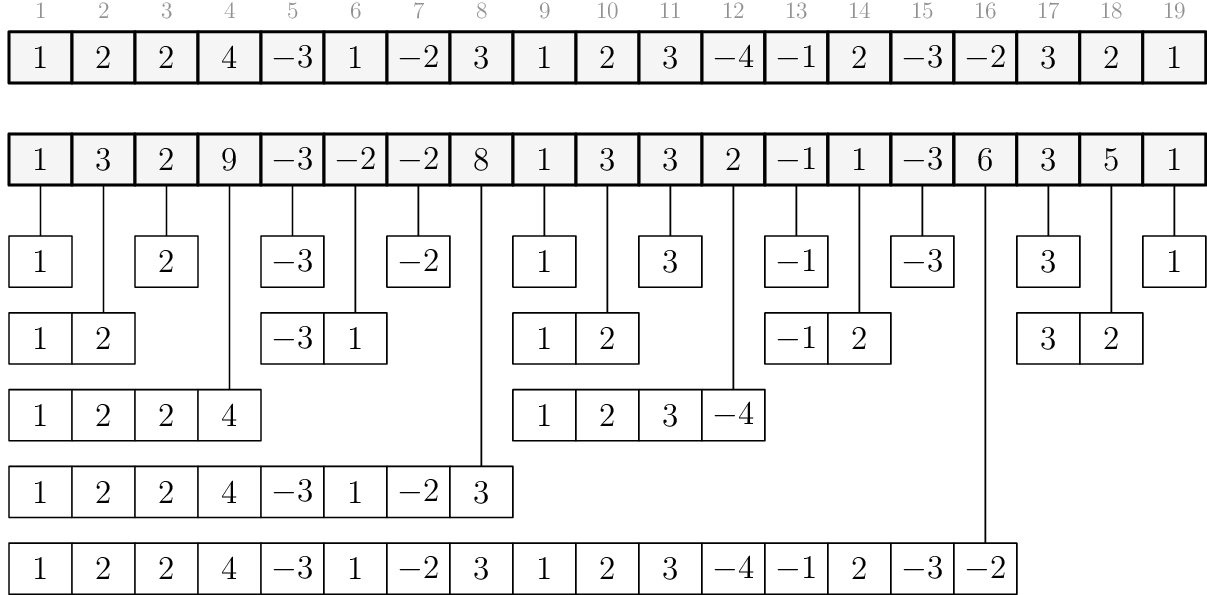
\includegraphics[width=\textwidth]{fenwick1.png}
\end{figure}
\end{frame}

\begin{frame}{Fenwick tree · prefix sum}
\begin{block}{Compute prefix sum}
The prefix sum $a[1] + \dots + a[i]$ can be calculated as follows:
$$prefix(i) = \begin{cases}
0 & \mbox{if } i = 0\\
ft[i] + prefix(i - lsb(i)) & \mbox{otherwise}
\end{cases}$$
It can easily be shown that the number of terms in this summation is equal to the number of ones of $i$, which means, $\mathcal{O} (log~n)$.
\end{block}
\begin{block}{Example}
See next slide: calculate
$$
prefix(13) = ft[13] + prefix(12) = \dots = ft[13] + ft[12] + ft[8]
$$
\end{block}
\end{frame}

\begin{frame}{Fenwick tree · prefix sum}
\begin{figure}
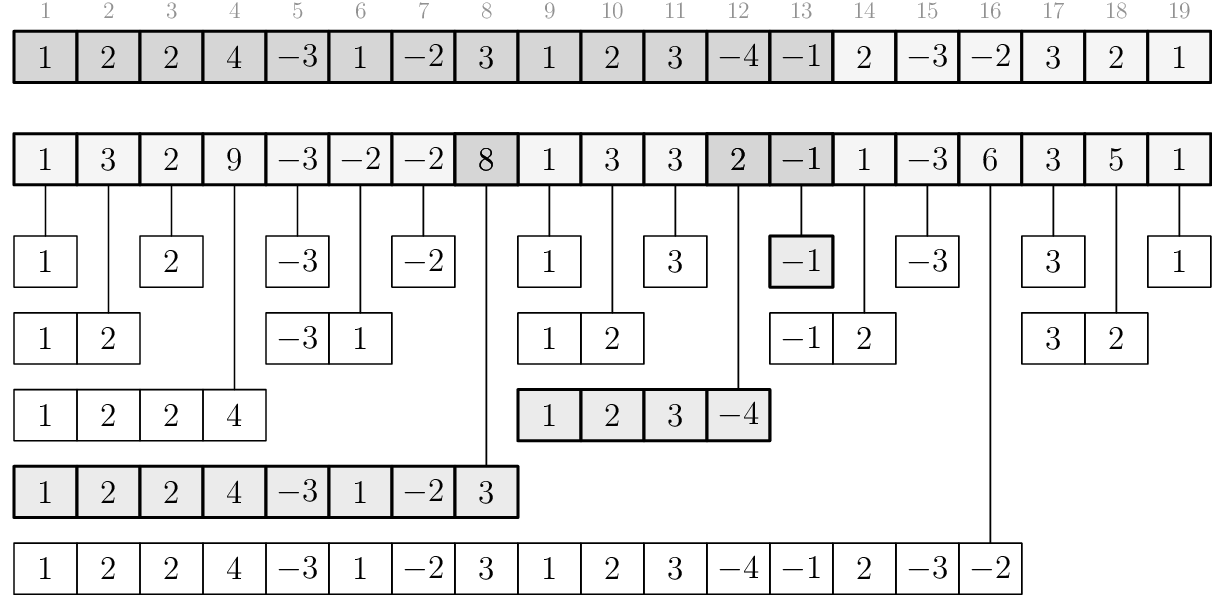
\includegraphics[width=\textwidth]{fenwick2.png}
\end{figure}
\end{frame}

\begin{frame}[fragile]{Fenwick tree · range query}
\begin{lstlisting}
#define lsb(x) (x & (-x))

int prefix_sum(size_t k) {
	int ans = 0;
	for (; k != 0; k -= lsb(k)) {
		ans += ft[k];
	}
	return ans;
}

int sum(size_t a, size_t b) {
	return prefix_sum(b) - prefix_sum(a - 1);
}
\end{lstlisting}
\end{frame}

\begin{frame}{Fenwick tree · point update}
\begin{block}{Compute point update}
We want to increase the element $i$ by a value $\delta$. To update an element of the original array we need to update $O(log~n)$ elements of the Fenwick tree, as follows:
\begin{gather*}
i_1 = i ~~~~~~~~~~~~~~~ ft[i_1] += \delta \\
i_2 = i_1 + lsb(i_1) ~~~ ft[i_2] += \delta \\
\dots
\end{gather*}
until $i_k <= n$
\end{block}
\end{frame}

\begin{frame}{Fenwick tree · point update}
\begin{figure}
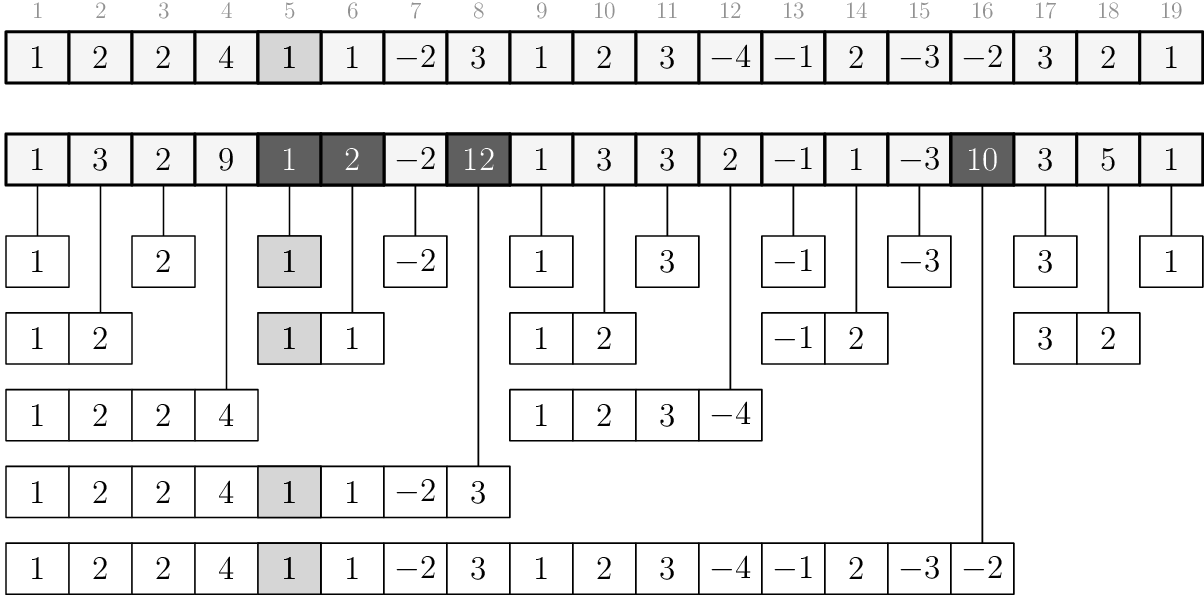
\includegraphics[width=\textwidth]{fenwick3.png}
\end{figure}
\end{frame}

\begin{frame}[fragile]{Fenwick tree · point update}
\begin{lstlisting}
void update(size_t k, int delta) {
	for (; k <= n; k += lsb(k)) {
		ft[k] += delta;
	}
}
\end{lstlisting}
\end{frame}

\begin{frame}{Fenwick tree}
\begin{block}{Final remarks}
\begin{itemize}
\item Initialize a Fenwick tree in $\mathcal{O}(n \cdot log ~ n)$  by repeatedly calling the update function.
\item Fenwick tree could be made zero-based tweaking the implementation of the interface.
\item A way smarter trick is to use a Fenwick tree to support \textbf{point query and range update}.
\end{itemize}
\end{block}
\end{frame}

\begin{frame}{Fenwick tree for range update}
\begin{block}{Problem}
We are given an array $P$ of $n$ integers and
\begin{itemize}
\item $k$ queries of the form: "given an integer $\delta$; $l$ and $r$, $l < r$, assign $P[l] += \delta; \dots; P[r-1] += \delta$"
\item $h$ queries of the form: "given $x$, retrieve $P[x]$".
\end{itemize}

Queries of the two types may be interleaved in any order.
\end{block}
\end{frame}
\begin{frame}{Fenwick tree for range update}
\begin{block}{Idea}
\begin{itemize}
\item Given an array $a$ of length $n$, start by creating the array of the finite difference $d$, s.t.
$$
d[i] = \begin{cases}
a[i] & \mbox{if } i = 1\\
a[i] - a[i-1] & \mbox{otherwise}
\end{cases}
$$
\item In the array $a$, point query can be done as follows: $a[i] = d[1] + \dots + d[i]$
\item In the array $a$, range update (add $\delta$ between $l$ and $r$) can be done as follows: $d[l] += \delta$, $d[r + 1] -= \delta$.
\end{itemize}
\end{block}
\end{frame}

\begin{frame}{Fenwick tree for range update}
\begin{block}{Build}
Simply, create a fenwick tree on the finite difference array $d$. Note that:
\begin{itemize}
\item a point query on $a$ corresponds to a range query (range sum) on $d$
\item a range update (range sum) on $a$ corresponds to a point update on $d$.
\end{itemize}
\end{block}
\end{frame}
\begin{frame}[fragile]{Fenwick tree for range update}
\begin{figure}
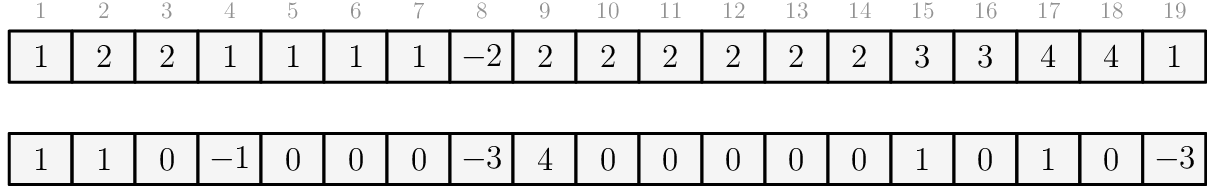
\includegraphics[width=\textwidth]{fenwick4.png}
\caption{Array $a$ (above), finite differences array $d$ (below)}
\end{figure}
\begin{figure}
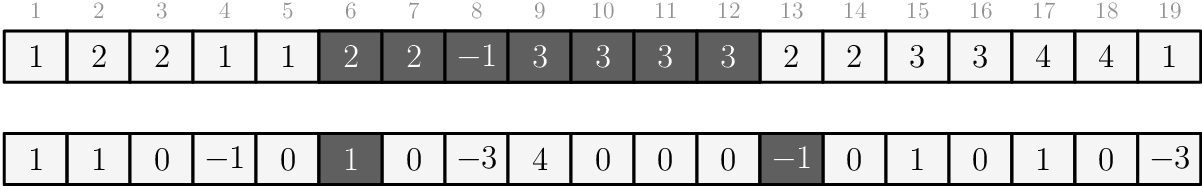
\includegraphics[width=\textwidth]{fenwick5.png}
\caption{Range update: $\delta = 1, l = 6, r = 12$}
\end{figure}
\end{frame}
\end{document}